% Copyright (c) 2014,2016 Casper Ti. Vector
% Public domain.

\chapter{PKI与区块链技术}


% Copyright (c) 2014,2016 Casper Ti. Vector
% Public domain.

\section{PKI}

本小节将对PKI系统进行详细介绍,首先从系统架构对PKI进行解析,阐述系统中包含的组成部分和各自的功能;其后将对证书进行介绍,包括证书的结构以及证书的生命周期;最后对本系统存在的问题以及相应的解决方案进行简要叙述。

\subsection{PKI系统架构}


PKI框架中包括安全和操作策略,安全服务以及支持公钥密钥和证书管理的交互式协议。公钥和对应证书的生成、分发和管理将通过授权机构(CAs)、注册机构(RAs)和目录服务来完成\cite{weise2001public},它们将会建立等级信任或者说信任链。以上提到CAs、RAs和目录服务可以将数字证书用于鉴定不同实体的身份,而PKI拥有如此架构的目的是为了能支持并完成数据、凭证在各种不安全环境下的安全交换。

在PKI中主要涉及的实体和相关组件如图\ref{fig:pki}所示。

\begin{figure}[htbp]
 	\centering
 	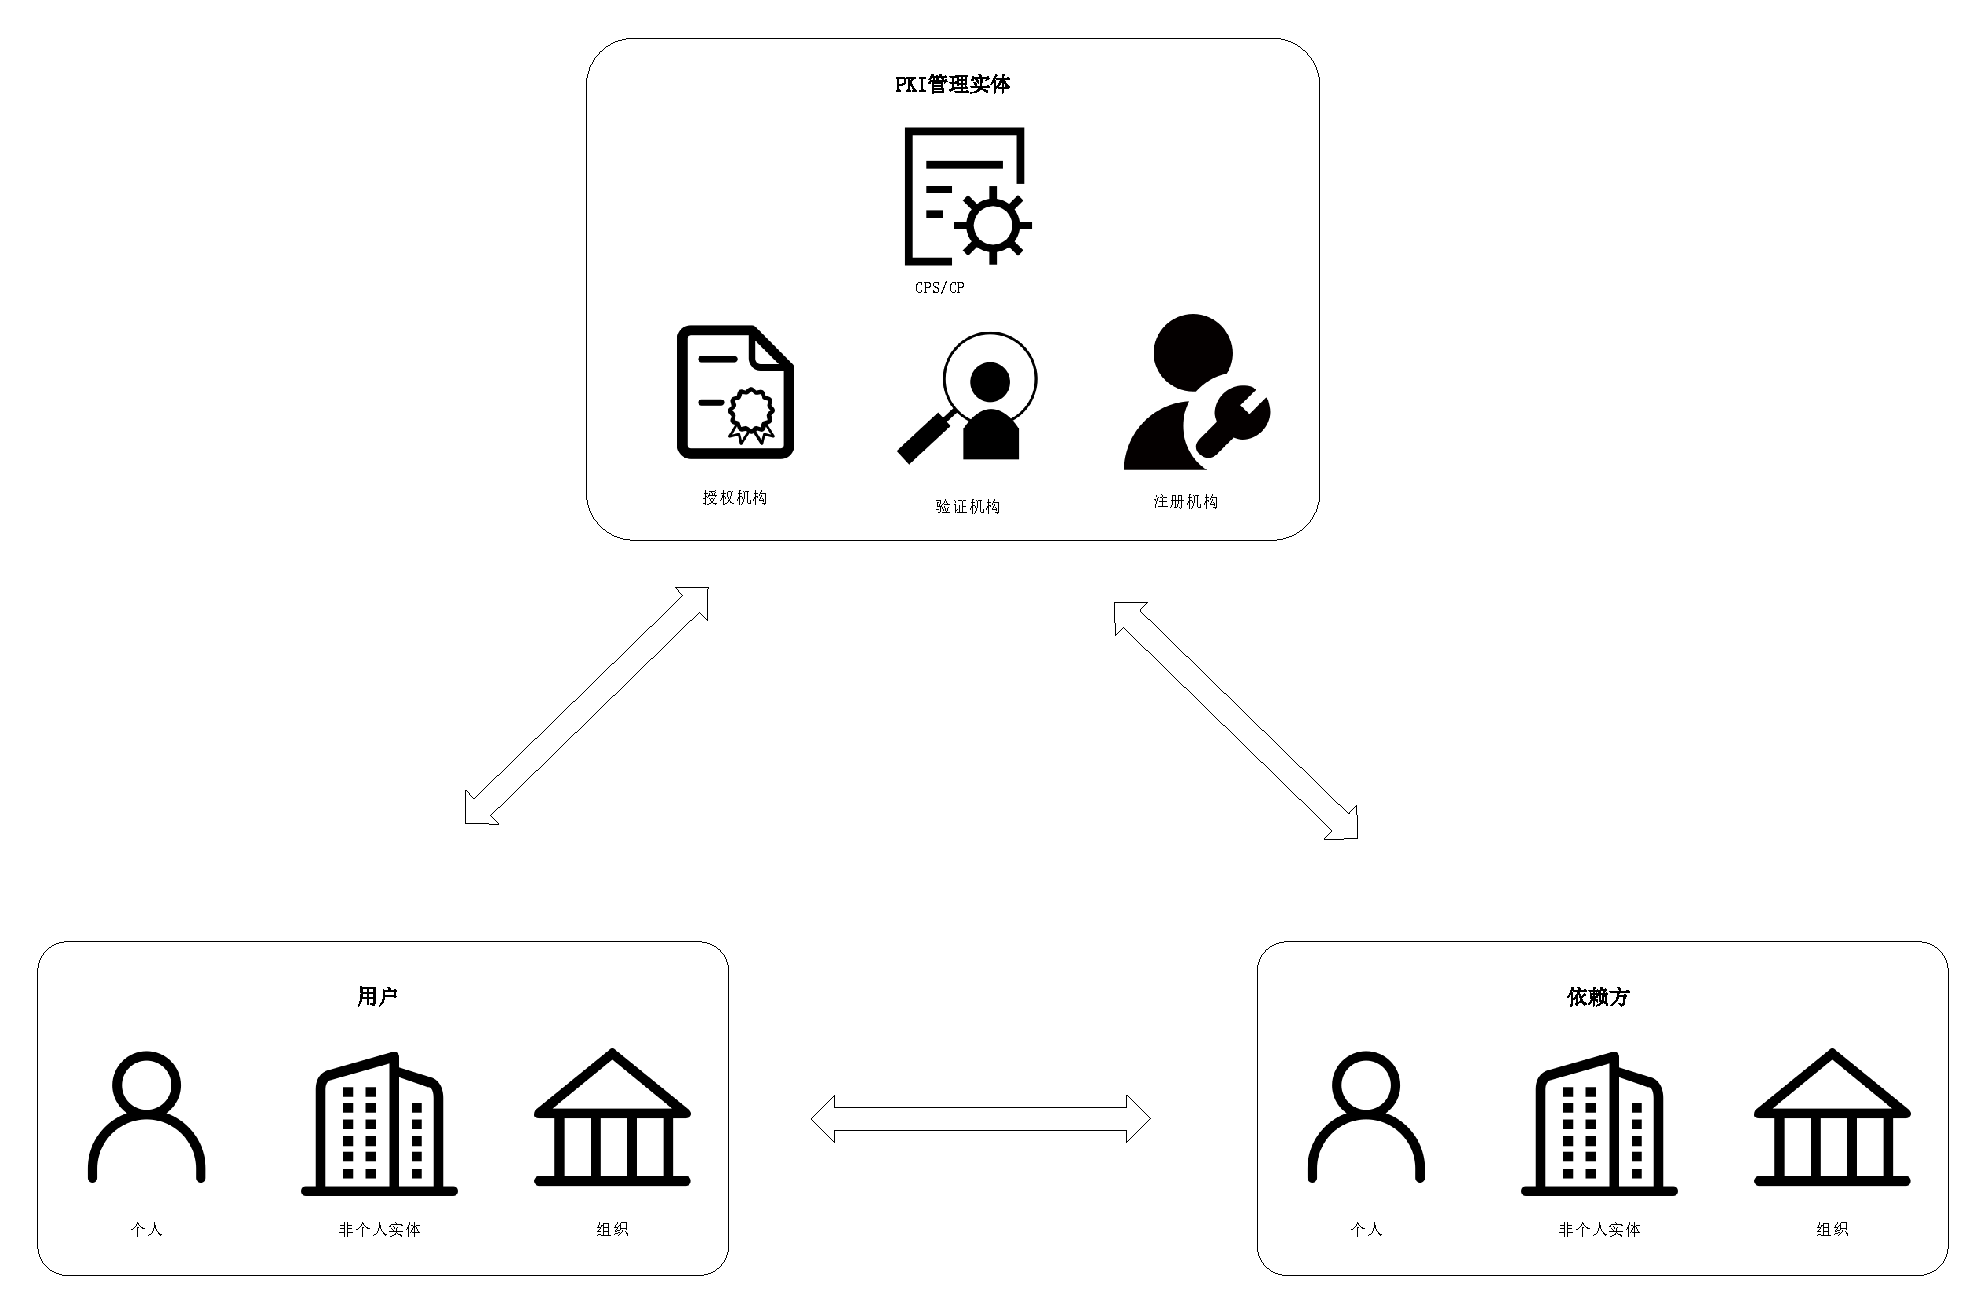
\includegraphics[width = 1\textwidth]{img/pki}
 	\caption{PKI实体和组件}\label{fig:pki}
\end{figure}



\subsection{证书}

\subsubsection{证书的结构}

% 数字证书作为PKI密钥管理服务中的公钥载体,通过授权机构对其的生成、发布、撤销来提供密钥管理服务。数字证书是一个由授权机构CA签名的数字文本,其中包含了证书申请者的身份信息比如实体的名称、电子邮件等,以及公钥信息。数字证书就像身份证一样,是包含第三方(即授权机构)签名的身份证明,依赖方可以通过对证书上面签名来判断身份是否真实效性。

在PKI的发展历程中,存在着多种数字证书的类型,每种类型的证书应用在不同的场景之中,因此也拥有各自独有的格式。目前最为通用的证书标准为X.509,该数字证书标准由国际电信联盟(InternationalTelecommunication Union, ITU)制定,于1988年公布最初版本。此标准的证书最为核心的部分是公钥和用户标识符,同时,X.509公钥证书中也可以包含证书版本号、序列号、签名算法标识、签发者名称、证书持有人名称和证书有效期等信息。X.509证书标准的最新版本是X.509 v3,在该版本中定义了数字证书的扩展信息,使得数字证书的功能可以进一步扩展,具有更大的灵活性,当数字证书在特殊应用环境下使用时,该扩展信息还可以起到传递附加信息的作用。

X.509 v3版本的数字证书结构如图\ref{fig:certificate}所示。

\begin{figure}[htbp]
 	\centering
 	\includegraphics[width = 0.8\textwidth]{img/certificate}
 	\caption{X.509数字证书结构\cite{fredriksson2017distributed}}\label{fig:certificate}
\end{figure}


\subsubsection{证书的生命周期}


证书作为包含公钥、数字签名以及一些其它附带信息的数字文档,在PKI系统中充当着公钥交换、存储和使用的介质。了解证书的申请、签发和使用流程,可以明白PKI系统的是如何运作的,并从中发现可能存在的问题。

证书的声明周期从用户提交准备的证书签发请求(CSR)并提交给其选择的CA开始。CSR中包含了用户的公钥和需要纳入的信息,并通过签名的方式表明对相应私钥的所有权。同时,CSR可以携带额外的信息元,但在实际使用过程中并没有全部使用。授权机构可以对CSR中的内容进行重写,放置一些其它的信息在证书中。

其后CA遵循验证流程,对用户进行身份验证。待成功完成验证之后,CA将签发证书,同时提供验证至根证书的所有中间证书。得到证书后,用户就可在证书过期之前使用证书。如果证书对应的私钥泄露,证书将可以被吊销,该过程和证书签发的过程类似。

对于Internet PKI系统而言,根据以上证书流转流程,证书的生命周期如图\ref{fig:cert_lifecycle}所示.

\begin{figure}[htbp]
 	\centering
 	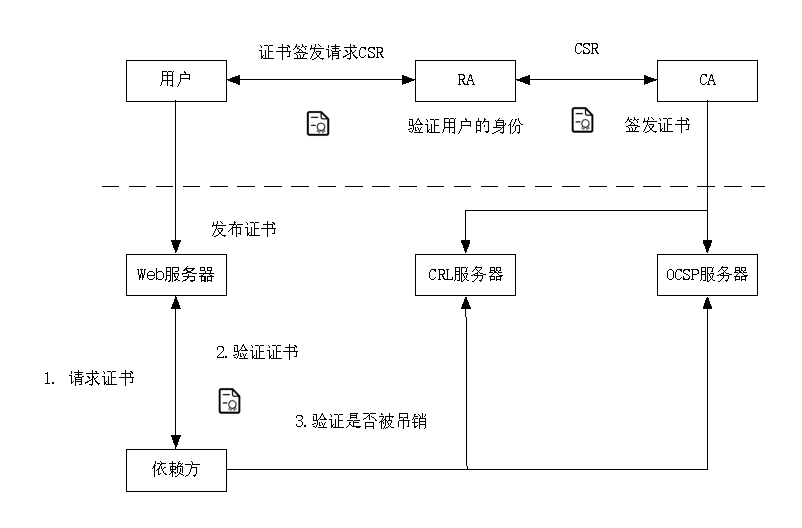
\includegraphics[width = 0.8\textwidth]{img/cert_lifecycle}
 	\caption{证书的生命周期}\label{fig:cert_lifecycle}
\end{figure}

\subsection{系统中存在的问题}

从安全的角度来看现有Internet PKI系统,其中存在着大大小小的各种问题,在本小节中,将对这些存在的问题进行简要概述。

当Web安全在1995年刚开始被谈及时,当时的互联网和现在是具有很大差异的,它的重要性并没有现在这么强。随着互联网的蓬勃发展,加密安全成为了商业中必备的一部分,关乎这一个企业的生死。现有的PKI系统和当初设计的目的是一致的,即为上电子商务操作提供足够的安全保障,更进一步可以说PKI系统希望提供商务安全。这种安全可以通较少的资金、更快的网页获取速度、可接受的不安全操作和不对用户做过多的限制来完成。本系统由CAs、寻利的商业实体和希望扩大市场份额的浏览器供应商一起来组成。

CA在本系统中充当着信任的基础,其每年签发了数百万计的证书,这些证书将在互联网中流通并使用。虽然这个系统正在正常的运转着,但是证书的安全性并没有想象中那么好。同时,在不那么完美的条件下,有时候用户还需要对申请的证书进行付费,然而并不是所有用户都愿意为之付出代价的,很简单的一个原因就是他们在付费之后希望得到完美的安全性保障。

在该系统中,存在着以下几个方面的问题\cite{ristic2014bulletproof}:


\begin{itemize}
	\item

	\noindent\textbf{域名权利过弱}

	在PKI系统中最大的问题是任意CA在未经域名同意的情况下就可以对其签发证书,导致这个问题的主要原因是系统需要对CA给予相当高的信任,但是没有相关的技术策略去避免CA的疏漏和安全隐患。当CA数量比较少的时候,这个问题并没有那么严重,但是当下有数以百计的CA存在,很难保证每一个授权结构都不会存在不端行为或者不当的安全配置。一个系统的安全性取决于该系统最薄弱的环节,而PKI系统中存在着各种潜在的薄弱环节。虽然所有的授权机构都会接收到审计,但是审计的质量却各不相同。例如在2011年DigiNotar由于自身安全性问题就被黑客攻陷,签发了数百个虚假证书,造成极其恶劣的影响,最后导致自身倒闭。

	同时,另外一个存在的问题是CA是否可以给予信任,它们能否在不需要监督的情况下为了公众的利益去做好自己的本质工作。这些被信任的CA可能在面对商业利益的时候放弃公众所需要的安全。例如在2012年Trustwave承认其签发了低级别的假冒证书用于流量检查。虽然Trustwave是唯一公开承认自己做过类似事情的CA,但大家相信这样的事情肯定大量存在。

	政府也可能会滥用PKI系统签发的虚假证书,完成对任意域名的假冒。公众无法确保CA不会作为政府的前线,即使不是也无法保证这些CA不会被迫签发虚假证书。



	\item

	\noindent\textbf{没有信任灵活度}

	另外一个重要的问题是本系统缺乏信任的灵活度。依赖方将会存储一系列信任的根证书,一个CA只存在信任与否,并不存在中间地带。理论上,依赖方可以移除任何对任意CA的信任,实际上这种情况只会在CA很小或者其已经被攻陷的时候发生。一旦一个CA签发了大量的证书,其将由于自身的大体量不会被撤销。

	一些小的改进措施在逐渐被提出,例如对具有过失行为的CA不再信任,但是其之前签发的证书仍然可以被使用。

	\item

	\noindent\textbf{域名验证过于简单}

	DV证书的签发是基于域名的WHOIS协议查询域名拥有者信息来完成的,即说大部分验证是通过邮件来完成的,而其本身的安全性就存在问题。如果域名被黑掉或者相应的邮箱密码被获取,那么就可以得到给域名的DV证书。同时通过拦截CA端验证信息也可以发起攻击。



	\item 

	\noindent\textbf{客户端验证不完整}

	在一般情况下,对吊销证书的检查并没有那么严格,大多数情况都不能正常的工作。在2011年中有很多这样的例子,依赖方不得不将被泄露的证书通过特殊通信方式下载并存储在黑名单中,来保证吊销查询是可靠的。

	这样做的原因主要包括以下两点,首先将吊销信息发送各个系统需要一定延时,在基准规则中允许CRL和OCSP的信息在10天是有效的,也就是说至少需要10天才能保证吊销信息被完全扩散出去;其次软失败机制在所有的浏览器中被使用,当依赖方在查询吊销信息时,如果没有收到查询回复时将任务证书未被吊销,一个主动的网络攻击者将可以轻易的拦截OCSP的请求,保证被吊销的证书可以完美的被使用。

	由于以上的原因,Chrome开发者取消证书吊销的检查,除非是EV类型的证书。对于重要的证书,例如中间证书,其将依赖于CRL信息的吊销通道查询相关信息。一种可能的解决方案是使用Must-stale的方案来保证证书的有效性。

\end{itemize}


\subsection{已有的改善措施}

为了解决X.509 PKI中的安全问题并削弱对CAs的信任,一系列的方案被提出来,本小节将对这些方案进行分类并简要叙述。



根据PKI中存在的主要三方实体域名、CA和客户端,可以对现有的方案进行分类,如图\ref{fig:Classification_of_PKI_proposals}所示。

\begin{figure}[htbp]
 	\centering
 	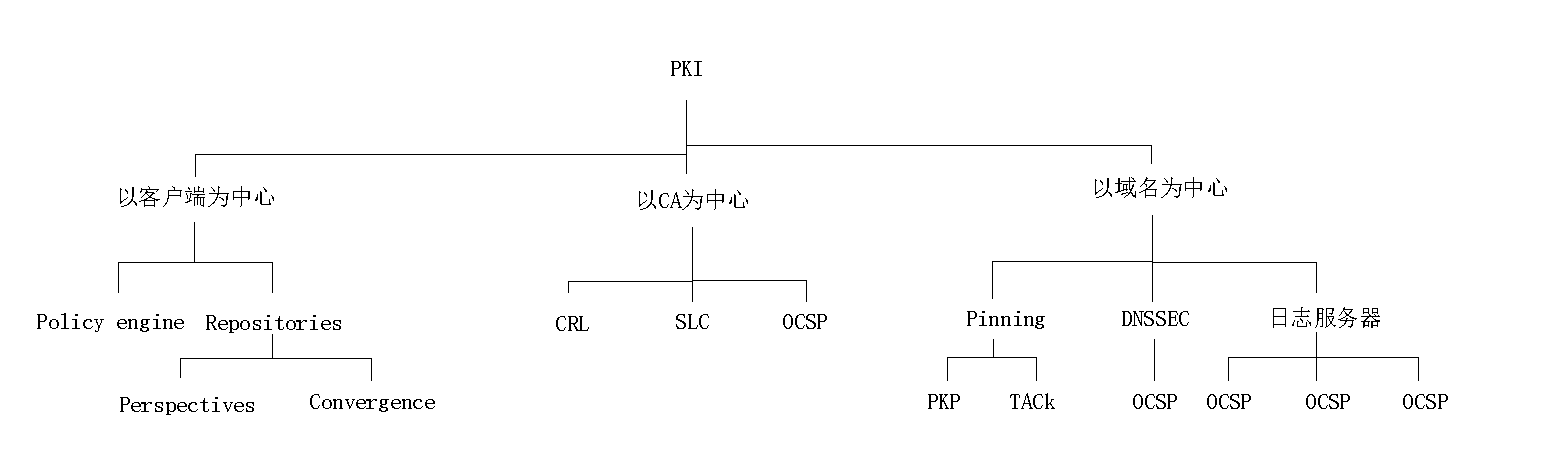
\includegraphics[width = 1.0\textwidth]{img/Classification_of_PKI_proposals}
 	\caption{PKI方案分类}\label{fig:Classification_of_PKI_proposals}
\end{figure}



\subsubsection{以客户端为中心的方案}

这类方案希望在客户端接受证书之前,可以更加准确的验证证书的有效性。Policy engine\cite{abadi2013global}的方案允许客户端在本地制定信任决策,比如支持的密码算法,证书的一致性性等。

有一些其它的方案希望构建一个公共的域名证书存储厂库,使得客户端可以在接受到域名证书之后与厂库中的证书进行对比,确定证书的正确性,Perspectives\cite{wendlandt2008perspectives} 和 Convergence\cite{convergence}就属于这类方案。

以客户端为中心的方案并不需要对服务端进行的改动,但是其需要客户端建立额外的连接去查询资源厂库,这将在一定程度上降低建立HTTPS的速度。


\subsubsection{以CA为中心的方案}

X.509 PKI包含了证书吊销列表(CRL)标准\cite{cooper2008internet},希望防止客户端与一个使用已经被吊销证书的域名之间建立TLS连接。但是这需要保证客户端需要能随时的访问到CRLs。为了进一步解决在线验证的问题,在线证书状态协议(OCSP)\cite{myers1999x}允许客户端通过CA的OCSP服务器去检查域名证书的状态。但是OCSP也拥有如安全、隐私、性能方案的顾虑。另外一个解决方案是短期证书(SLC)\cite{topalovic2012towards},该方案希望签发短生命周期的证书,让域名定期的更换证书。SLC希望带来和OCSP类似的好处,但是不需要在线验证。以证书为中心的方案严重依赖于浏览器去检测和拉黑被攻陷CA签发的证书,这是这类方案的最大缺陷。


\subsubsection{以域名为中心的方案}


第三类方案允许域名拥有者积极控制和保护他们的证书而不被CA端的潜在问题所威胁。这些方案又可以分为以下三类:pining、DNSSEC、日志服务器。

1. Pinning-based(公钥固定)

如Public Key Pining(PKP)\cite{evans2015public}和Trust Assertions for Certificate Keys(TACK)\cite{topalovic2012towards}等Pinning的方案希望域名宣称自己使用的密钥,以便客户端收到的密钥是否正确。但是这类方法有自己的安全缺陷,比如在第一次访问域名的时候无法给予安全保护。

2. DNSSEC-based

这类方案的全称叫基于DNS的命名实体鉴权(DANE)\cite{schlyter2012dns},希望域名的所有者可以在DNSSEC实体上放置证书相关的特殊声明,例如可以为其签发证书的CA名单、声明接受的证书或者是声明验证证书有效性的站点,但是DANE的安全性严重的依赖于DNS操作的安全性。


3. 日志服务器

另外一种使用比较多的方法是通过日志服务器的方案来记录CA的行为,为域名拥有者提供公共的、可审计的CA行为日志,监督CA的行为。例如 Sovereign Keys (SK)\cite{eckersleysovereign}要求域名拥有者生成一个主密钥对来完成对TLS公钥的签名,并且将其主公钥以只读和只可追加的方式记录在时间服务器上。然而,SK需要客户端查询服务器,增加了延迟并牺牲了隐私。

证书透明(CT)\cite{laurie2013certificate}的方案允许每个域名将自己的证书注册记录到一个公共日志服务器上,该服务器使用默克尔哈希树的结构来存储这些证书,并保证只能追加的性质。该服务器将返回一个不可否认的证书审计证明给域名,域名使用证书和该证明来完成与客户端TLS连接的建立。但是,本方案并不能防止当一个攻击者攻破了CA并创建并注册一个虚假的证书的情况,CT并不能阻止客户端接受这类证书。由于证书透明在设计过程中并没有强调证书的吊销,相应的证书吊销透明(RT)\cite{laurie2012revocation}也被提出。为了提高CT对证书吊销的效率,证书签发吊销透明(CIRT\cite{ryan2014enhanced}方案被提出。

另外一种基于日志服务器的方案称作可审计密钥设施(AKI)\cite{kim2013accountable},该方案希望保护域名和客户端遭受到单点失败攻击,比如某个CA的根密钥被泄露,通过制衡该系统中各个实体,AKI在保持高效处理证书操作的情况下,成功的将信任分散到了多个实体,并可以检测出实体的恶意行为。




% vim:ts=4:sw=4


\section{区块链技术}




区块链技术作为当下作为最火热的技术之一,从09年以比特币的形式出现在人们的视野中,就一直被大家关注和讨论。本章节将从比特币出发,给出区块链技术的整体概况,其后将对区块链技术中的核心部分共识机制和智能合约进行简要介绍,最后简单列举区块链技术典型应用场景。

\subsection{比特币与区块链技术}


比特币作为一个P2P电子货币系统,是由中本聪在08年中的一篇论文中提出\cite{nakamoto2008bitcoin},整个系统如下图\ref{fig:bitcoin}所示。

\begin{figure}[htbp]
 	\centering
 	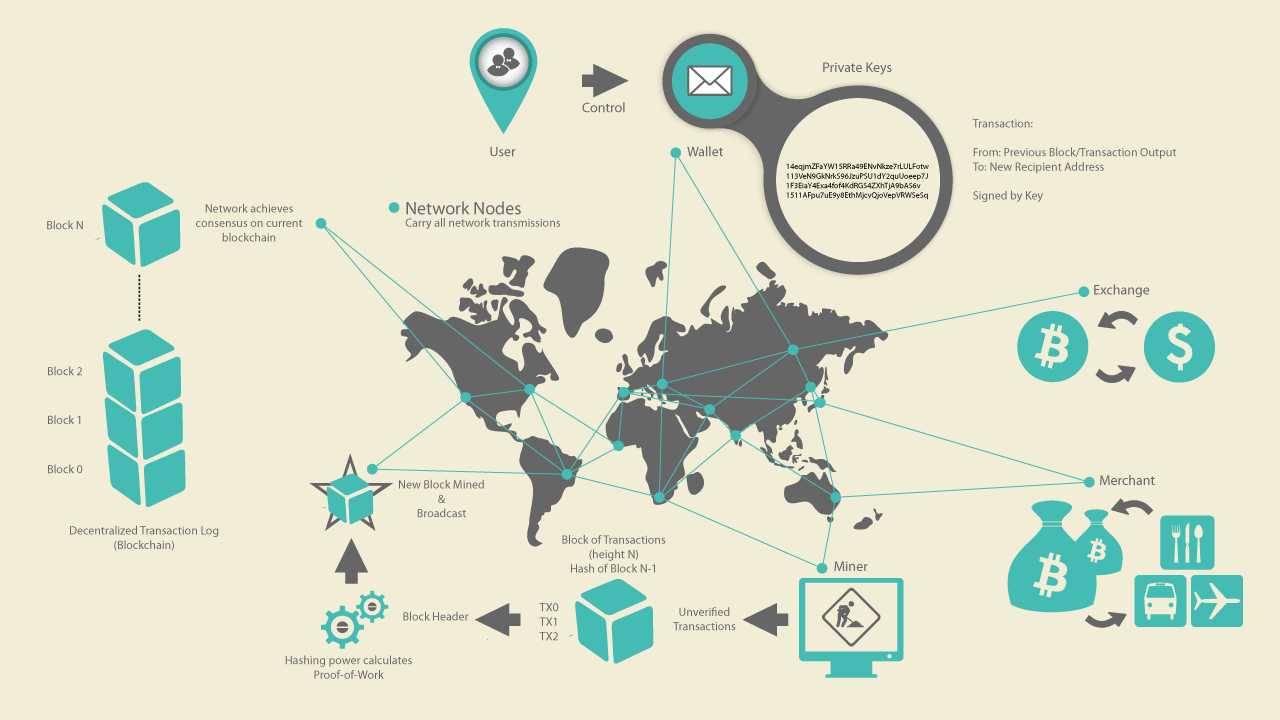
\includegraphics[width = 1\textwidth]{img/bitcoin}
 	\caption{bitcoin 概述\cite{antonopoulos2014mastering}}\label{fig:bitcoin}
\end{figure}

比特币是构建在一个P2P网络上的数字货币系统,由拥有公私钥对的用户、网络中传播的交易和通过计算竞速的生成块的矿工共同组成。在该系统中,用户使用私钥完成对已有资产(比特币)的转移,形成有效的交易递交到比特币构建的去中心化网络中;而矿工作为网络中区块的生成者,为了获得建块的奖励和纳入交易后的交易费,将有效的交易纳入新的区块,并使用自己的计算资源不断尝试下一个区块的构建;当某个矿工率先完成下一区块的创建时,会将新的区块立即广播给网络中的其它矿工,待他们验证通过后会在被接收的区块上进行一下区块产生的竞速过程。


% \noindent\textbf{区块结构}


\begin{figure}[!htbp]
 	\centering
 	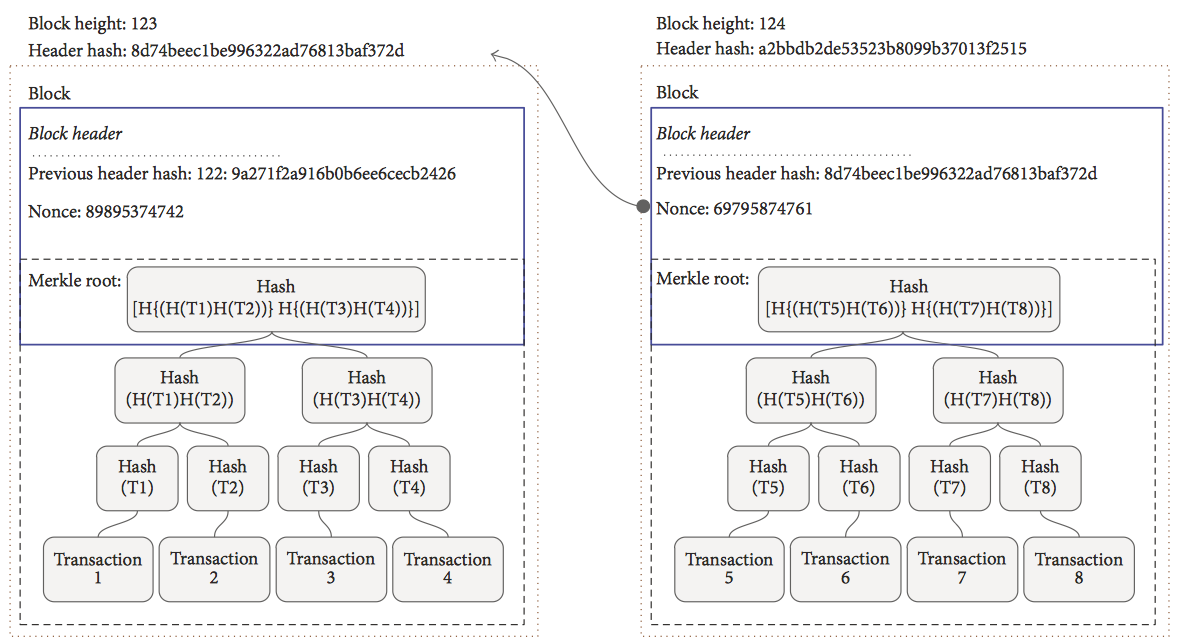
\includegraphics[width = 0.8\textwidth]{img/block_structure}
 	\caption{区块结构}\label{fig:block_structure}
\end{figure}

区块作为比特币中交易记录的载体,通过纳入上一区块哈希的方式保持所有区块的连贯性,其结构如图\ref{fig:block_structure}所示。一个区块由区块头和交易两部分组成,交易部分包含了本区块的所有交易的详细内容。在区块头中主要包含了上一区块的哈希值,用于指明上一区块;以及本区块中所有交易组建Merkl树的根和通过大量计算得到一个工作量证明的nonce值。区块创建过程即是矿工在区块链中所谓的挖矿,而挖矿的本质其实就是计算区块当中的nonce值。





% \noindent\textbf{区块链技术架构}

% \begin{figure}[!htbp]
%  	\centering
%  	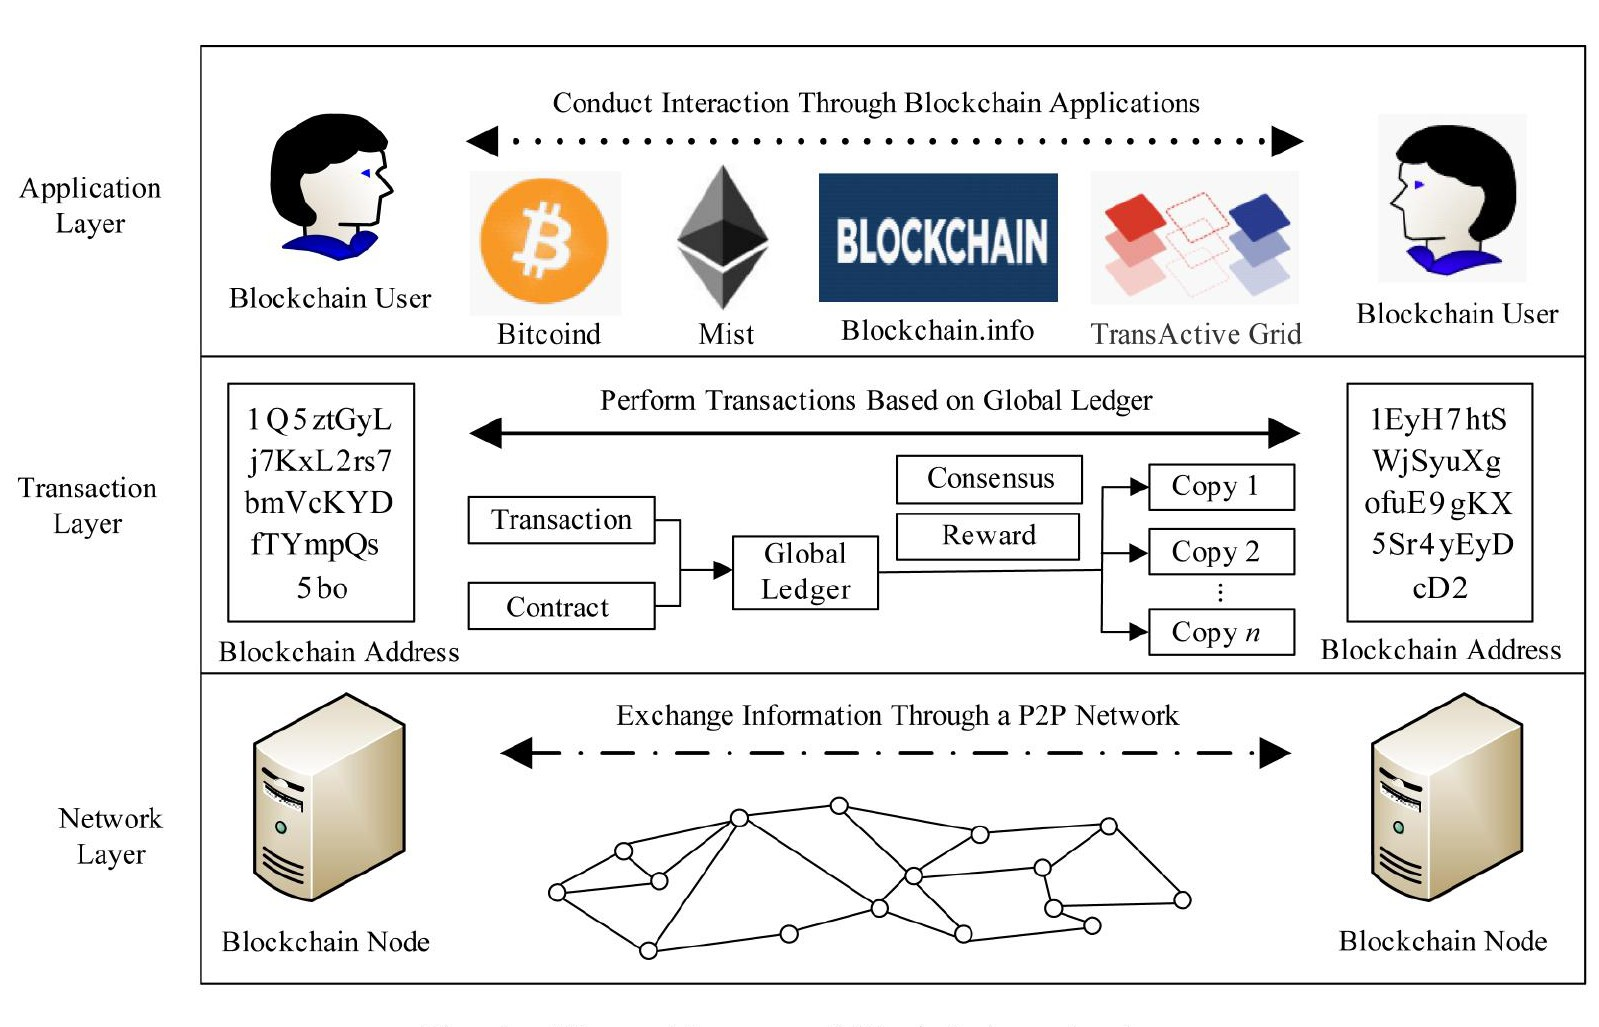
\includegraphics[width = 1\textwidth]{img/blockchain_framework}
%  	\caption{技术架构}\label{fig:blockchain_framework}
% \end{figure}


% \noindent\textbf{比特币交易}

% 比特币交易包含了多个输入和输出。每个输出通过一个两元组来表示$(a,V)$,其中$a$是发送比特币的数量,$V$是一个关于谁有权花掉这笔钱的声明。在比特币中,这个声明被称作$scriptPubKey$,它是由栈式非图灵完备语言书写的比特币脚本。交易的输入指向一个前面交易的输出,同时包含第二个脚本$scriptSig$,可以用于$scriptPubKey$的代码和数据。Coinbase交易不需要纳入一个先前的交易输出作为输入。

% 为了向Bob发送d个比特币,Alice需要Bob的ECDSA公钥$pk_b$,并将其哈希和发送的数量$d$以及一些其它的指令放置在$scriptPubKey$中作为一个交易的输出,当然,这笔交易需要至少需要$d$数量的比特币作为输入,如\ref{code:tx}所示。如果输入的金额大于输出的金额,而且交易提交者没有设置额外的转账地址的话,剩余的金额将会被作为交易费支付给将其纳入块的节点。一旦这笔交易被广播到网络中并收入到一个有效的块中,相应的比特币就属于Bob所有了。如果Bob想花掉这笔钱,他需要将这笔交易的输出作为新建交易的输入,并附带上包含$pk_b$对应私钥$pr_b$签名的$scriptSig$即可。

% \begin{lstlisting}[caption={比特币交易实例}, label=code:tx]
% Input:
%   Previous tx: 0205937d9faaa1a313b7826fdab...
%   Index: 0
%   scriptSig: odc23450cdf8cdc710e5e92af7647...

% Output:
%   Value: 500000
%   scriptPubkey: OP_DUP OP_HASH160 a45f275794fd2337ebf7ddd018c11a21fb6c283 OP_EQUALVERIFY OP_CHECKSIG

% \end{lstlisting}





\subsection{共识机制}

区块链网络中的节点需要对新生成块中的交易及顺序达成共识,从而达到相同的状态,否则任何节点都可以产生分支而导致分叉。如果网络中的节点各自拥有不同的状态,那么该网络就无法对所有操作做出相同的判断,这个系统就不能协同运行下去。在一个分布式的P2P网络中,在没有第三方协调分歧的情况下,就需要有一种机制来保证每个节点可以达到相同的状态,而区块链上的共识机制就解决这一问题的,保证网络中各个节点的一致性。

在理想的情况下,所有的验证节点对下一个区块中的交易顺序进行投票,根据大多数人的选择来确定下一区块如何产生。但是在一个公开且没有身份管控的开放网络中,任何人都可以自由的加入,将会遭受到女巫攻击\cite{douceur2002sybil}:单一节点可以拥有多个身份表示,通过控制系统中的大部分节点来左右网络向对自己有利的方向进行。也就是说,少数的个体可以通过女巫攻击完成对整个网络的控制。

比特币通过提高产生块的计算量来解决这一问题,使得在网络中添加多个实体并不能发起女巫攻击,因为对于单个实体而言,其计算资源是有限的。更具体一点,网络中的任意节点都可以去产生下一个块,但是其需要找到一个正确的随机值(nonce)填入到区块的头部,使得产生块的哈希拥有至少指定数量的前导零\cite{antonopoulos2014mastering}。任何节点都可以对这个问题进行尝试求解,也就是所谓的工作量证明(proof of work),来完成对下一区块的构建\cite{nakamoto2008bitcoin}。在该过程中使用的是单向哈希函数,当一个节点宣称自己找到一个解的时候,其它节点很容易的去验证是否符合要求,但在给出目标的时候却无法直接确定输入应该是什么,只能通过不断尝试来玩寻求答案。

依照上述方案,当网络中的节点同时计算出下一个块时,依旧有可能存在分叉的情况。但这种分叉并不会带来影响,因为比特币中的工作量证明机制规定节点应该在工作量最大的链上进行下一区块的产生,而两个分叉的区块基本上不可能同时产出下一个块,先产生块的分支将会成为网络中被网络中节点选中的链,会有更大的几率成为更长的链,这使得网络又恢复到了统一的状态。

在比特币中使用的哈希算法是SHA-256,其它的哈希算法如Blake-256和scrypt也在被使用,同时还有一些共识机制中混入多种哈希算法。

工作量证明的方式虽然简单有效,但是其需要很多计算资源才能进行区块的产生,并且大量的计算导致能源浪费。权益证明(proof-of-stake)\cite{vasin2014blackcoin}是另外一种替代POW的共识算法,根据节点的账户余额来决定下一块的生成权;与POW相比,POS拥有自己优势和劣势,并且其应用在起来也十分的复杂。

空间和时间一直是两个对立面,很多算法为了降低时间复杂度不得不牺牲大量空间,最近另外一种名为容量证明共识机制也被很多研究者讨论。容量证明\cite{ateniese2014proofs}的原理是需要大量的空间去寻求一个谜题的答案,如果能够给出给定问题的解,那么证明其拥有住够多的空间。具体而言,容量证明会基于矿工的公钥进行初始化,这将耗费矿工大量的磁盘空间,并将初始化的相关内容存储在矿工的计算机中;其后在挖矿的过程中,需要对区块链上的谜题进行求解,每个矿工根据本地存储相关内容,通过对磁盘的扫描获得对应的解,并完成区块的生成。以上两个过程分别是初始化过程和挖矿过程,值得注意的是,初始化过程是一个很慢的过程,单个矿工可能需要耗费数天来完成初始化,这样做的目的为了防止提过快速的计算硬件来替代存储;对于挖矿过程而言,是一个极快的过程,只需要对磁盘进行扫描即可,并不需要像工作量证明那样耗费大量的能源。随着硬件的运算能力越来越高,工作量证明的方式从原有的CPU挖矿已经转变成ASIC挖矿,使用容量证明的方式可以抗ASIC挖矿,这也是广大研究者对其感兴趣的原因。


\subsection{智能合约}

智能合约的概念于1994年被Nick Szabo提出\cite{szabo1996smart},是一种旨在以信息化方式传播、验证或执行合同的计算机协议,允许在没有可信第三方的情况下进行交易,完成的交易将是可追溯且不可逆的。Szabo建议将合同的条款转换成代码,并将代码放置在特定的软件或者硬件环境中运行,减少交易方对可信中介的依赖,以及第三方的避免不端行为或者意外操作。由于一般网络中缺少可信的执行方,使得智能合约在提出之后并没有被广泛应用,而区块链提供了可信的执行环境,因此智能合约在区块链出现之后逐渐被火热起来。

在区块链的环境下,智能合约是存储在区块链上的脚本。由于智能合约存在于链上,每个智能合约会拥有独一无二的地址,并通过发起对相应地址的交易来实现对智能合约的调用。收到出发交易后,智能合约将会在每个节点上按照合约的设定,自动独立地执行合约内容。事实上在每个节点上都运行着一个虚拟机(VM)来执行合约代码,区块链网络充当着分散式VM的角色。

区块链技术最开始仅仅是用于转账交易的记录,而智能合约的应用使得在区块链上可以开发出功能更加丰富的应用。用户根据自身的需求,使用智能合约语言将需要的逻辑操作编写成合约代码,并以交易的形式发布到区块链上,该步骤即为智能合约的书写和部署。当智能合约存在于区块链上之后,用户就可以向合约的地址发送交易来调用合约,完成合约内容的执行,即智能合约的调用。


不同区块链平台合约语言的自身性质将决定智能合约能够实现的操作,如比特币上使用的基于堆栈的脚本语言,指令集小并且不支持循环等复杂运算,可以实现的功能就很有限。从以太坊之后的区块链平台,基本上都拥有图灵完备的合约语言,能够实现各种应用逻辑,极大的扩展了区块链本身的功能,可以应用在数字货币之外的场景。特别是对于金融领域、智能资产、托管支付等许多场景都能通过智能合约来实现。区块链为智能合约的执行提供了可信的环境,而智能合约则给区块链赋予了更加宽广的应用场景。



\subsection{与PKI相关的应用}




%turn a blcokchain into PKI
由于PKI系统中的信任是基于第三方中心化的CA,当单个CA被攻击之后,将会导致整个系统的处于危险之中,同事该系统中提供的服务都存在着单点失效(POF)的风险。一些研究希望通过将区块链技术应用在PKI系统中,弥补现有体系中的一些缺陷,例如在\parencite{baldi2017certificate}中,将撤销的证书存储在区块链上,提供更加可靠的证书验证服务,可以避免传统OSCP中单点失效的问题。IKP\cite{matsumoto2016ikp}方案利用以太坊智能合约,将PKI中证书相关的操作都转移到区块链上,记录证书的申请、签发以及吊销过程,让PKI中的各个步骤都是公开可审计的,此时区块链相当于是公开且不可篡改的日志服务器,供大家审计PKI系统中的所有操作。

%blockstack?? or ETHIKS or CONIKS


Certcoin\cite{fromknecht2014decentralized}借鉴Namecoin实现了一个基于区块链的PKI系统,其通过默克尔哈希树来完成对身份信息的存储并通过Kademlia DHT完成快速查询。Nidaba\cite{rystsovnidaba}则从分布式PKI的可扩展性和证书操作的代价出发,基于区块链提出了一套完整的架构;SCPKI\cite{al2017scpki}利用web-of-trust模型以及以太坊上的智能合约,提出了一种去中心化且透明的方案,保证异常证书被签发时能够及时的被检测到。



% vim:ts=4:sw=4























